% !TeX spellcheck = da_DK
\subsection{Filter}\label{Filter_afsnit}
\subsubsection{Teori og design}
%Efter signalet er blevet forstærket skal det filtreres, så alle de uønskede signaler kan dæmpes. Der benyttes kun et lavpasfilter, da det ønskede signal ifølge litteraturen kan ligge i frekvensområdet $0-10$Hz, som beskrevet i afsnit \ref{FilterAfs} på side \pageref{FilterAfs}. Jævnfør pilotforsøget i afsnit \ref{Sec:PilotforsoegKort}, side \pageref{Sec:PilotforsoegKort} blev der målt et signal i frekvensområdet $0-25$Hz og det frekvensområdet sættes derfor til $0-25$Hz, for at filtrere uønskede signaler fra. 
Filtre kan udarbejdes i aktiv og passiv form. Hvis signalet ligger i frekvensområdet under $1$MHz, anbefales det at benytte aktive filtre. Aktive filtre benytter operationsforstærkere, kondensatorer og modstande, hvor passive filtre benytter kondensatorer, modstande og spoler. \cite{Carter2013} Der findes flere forskellige typer filtre, heriblandt Butterworth-, Tschebyschev- og Besselfilter. Butterworthfilteret giver maksimal fladhed i pasbåndet og stopbåndet. Tschebyschevfilteret giver den hurtigste overgang fra pasbåndet til stopbåndet. Besselfilteret giver en lineær faserespons, hvilket vil sige, at fasen er lineær med frekvensen.\fxnote{NTK: Fasen angiver, hvor godt et signals frekvensspektrum bliver gengivet} \cite{Carter2013} I dette projekt anvendes et Butterworthfilter, da der ønskes maksimal fladhed i pasbåndet og stopbåndet\fxnote{NTK: Dette ønskes for at få en pæn overgang og der kræves ikke en hurtig overgang fra pasbånd til stopbånd}. De forskellige typer filtre fremgår på \figref{fig:type_filtre}.
\begin{figure}[H]
	\centering
	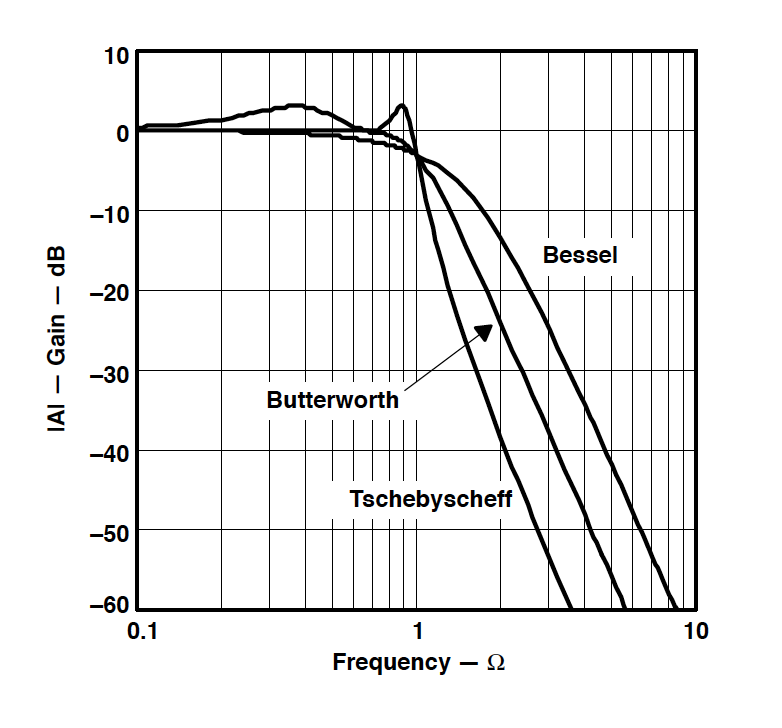
\includegraphics[scale=0.7]{figures/cProblemloesning/type_filtre.PNG}
	\caption{På figuren ses egenskaberne for de tre filtertyper: Butterworth-, Tschebyschev- og Besselfilter. \cite{Carter2013}}
	\label{fig:type_filtre}
\end{figure}
\noindent Når designet af filtret er valgt, findes der flere forskellige måder, hvorpå et filter kan implementeres. Eksempler på disse metoder er Sallen-Key topologien (SKT) og Multiple Feedback toppologien (MFT). SKT-metoden er den mest anvendte og tillader separate gain-indstillinger samt inverterende og ikke-inverterende konfigurationer, hvorimod MFT-metoden benyttes i filterdesign med høj gain-nøjagtighed (Q-værdi). I dette projekt benyttes en ikke-inverterende konfiguration grundet den høje indgangsimpedans i den ikke-inverterende terminal, hvorfor SKT-metoden er valgt. Herved forhindres det, at filtret loader fra de forrige blokke, jævnfør bilag \ref{Bilag:Pilotforsoeg}, side \pageref{Bilag:Pilotforsoeg}. Hvis der vælges et inverterende design for operationsforstærkeren i filterkonfiguration, vil blokken have en lav indgangsimpedans, hvorfor denne blok vil begynde at loade. Der kræves derfor mere strøm for at opretholde outputspændingsniveauet. \cite{webster2009,Carter2013,karni2014}

Jævnfør kravspecifikationer af lavpasfilteret i afsnit \ref{FilterAfs}, side \pageref{FilterAfs} kræves det, at filteret har en minimumsdæmpning af stopbåndet $(A_{min})$ på $14$dB og der accepteres en maksimal dæmpning af pasbåndet $(A_{max})$ på $3$dB. Derudover skal lavpasfilteret have en pasbåndfrekvens $(\omega_p)$ på $25$Hz, samt en stopbåndfrekvens $(\omega_s)$ på $45$Hz. På \figref{fig:Lavpasfilter_generisk} fremgår en illustration af, hvad de forskellige parametre beskriver. Ydermere skal filteret kunne modtage et signal i intervallet $\pm3$V. Dette afhænger af valget af operationsforstærker samt spændingsforsyning til denne. 
Til designet af filteret benyttes en operationsforstærker af typen TL$081$, som ifølge databladet vil give et arbejdsområde på $\pm13.5$V med en spændingsforsyning på $\pm15$V \cite{Corporation1995}. Operationsforstærkeren forsynes med en spænding på $\pm5.5$V jævnført afsnit \ref{Spaendingsforsying}, side \pageref{Spaendingsforsying}. Det forventes, at TL$081$ vil give et arbejdsområde på minimum $\pm3$V uden, at signalet klippes. %når der bruges en spændingsforsyning på $\pm5.5$V. 

\begin{figure}[H]
	\centering
	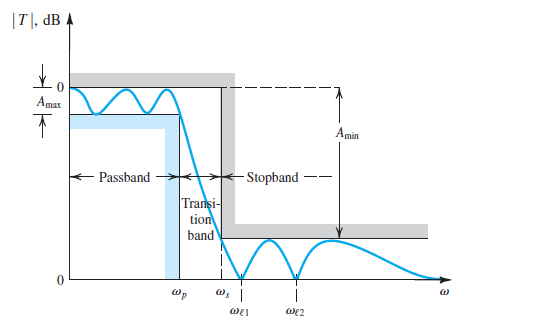
\includegraphics[scale=1.2]{figures/cProblemloesning/Lavpasfilter_generisk.PNG}
	\caption{På figuren ses et bodeplot af et lavpasfilter, hvor de fire karakteristika $(A_{min})$, $(A_{max})$, $(\omega_p)$ og $(\omega_s)$ er angivet. \cite{Carter2013}}
	\label{fig:Lavpasfilter_generisk}
\end{figure}
\noindent Med udgangspunkt i de enkelte parametre af lavpasfilteret kan den pågældende orden af filteret bestemmes vha. \eqref{eq:lavpasfilter} for overføringsfunktionen:
\begin{equation} \label{eq:lavpasfilter}
A(\omega_s) = 10 \text{log} \cdot \left[1 + \epsilon^2 \cdot (\frac{\omega _s}{\omega _p})^{2N}\right] 
\end{equation}

\noindent I \eqref{eq:lavpasfilter} betegner $A(\omega _s)$ den minimale dæmpning, der kræves af stopbåndet. $(\omega_p)$ og $(\omega_s)$ er pasbåndfrekvensen og stopbåndfrekvensen, som begge er angivet i Hz. N angiver filtrets orden, og $\epsilon$ er udtrykt ved \eqref{eq:epsilon}:
\begin{equation}\label{eq:epsilon}
\epsilon = \sqrt{10^{A_{max} / 10} -1}
\end{equation}

\noindent Lavpasfilterets orden kan herefter bestemmes, jævnfør værdierne fra kravspecifikationerne fra afsnit \ref{FilterAfs}, side \pageref{FilterAfs} ved at indsætte disse værdier i \eqref{eq:lavpasfilter}. Udregningerne vil se ud som følgende:
\begin{eqnarray}\label{eq:orden}
\epsilon = \sqrt{10^{3dB /10} -1} = 0.998 \\ 
14\text{dB} = 10 \cdot \text{log} \left[1 + \epsilon ^2 \cdot (\frac{45\text{Hz}}{25\text{Hz}})^{2N}\right] \\
\label{eq:orden3}N = 2.711 \approx 3
\end{eqnarray}
\noindent Det fremgår af \eqref{eq:orden3}, at lavpasfilterets er af $3$. orden. Filterets orden angives i hele tal og derfor afrundes resultatet. For at overholde kravene til lavpasfilteret afrundes ordenen opad. Af \figref{fig:SallenKey1} og \textbf{\ref{fig:SallenKey2}} fremgår hhv. et $1$. og $2$. ordens lavpasfilter designet efter SKT. \cite{Carter2013}
	
\begin{figure}[H]
	\centering
	\begin{minipage}[b]{0.45\textwidth}
		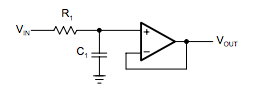
\includegraphics[width=\textwidth]{figures/cProblemloesning/Lavpasfilter1_teoretisk.PNG}
		\caption{På figuren ses en illustration af et $1$. ordens unity-gain Sallen-Key lavpasfilter, hvor værdien C er kondensatoren og R$1$ er modstanden. Filterkonfigurationen har en indgangsspænding, $V_{in}$, og udgangsspænding, $V_{out}$. \cite{Carter2013}}
		\label{fig:SallenKey1}
	\end{minipage}
	\hfill
	\begin{minipage}[b]{0.45\textwidth}
		\includegraphics[width=\textwidth]{figures/cProblemloesning/Sallenlavpas.PNG}
		\caption{På figuren ses en illustration af et $2$. ordens unity-gain Sallen-Key lavpasfilter, hvor værdien C er kondensatoren samt R$1$ og R$2$ er modstandene. Filterkonfigurationen har en indgangsspænding, $V_{in}$, og en udgangsspænding, $V_{out}$. \cite{Carter2013}}
		\label{fig:SallenKey2}
	\end{minipage}
\end{figure}

\noindent I designet af et $3$. ordens lavpasfilter designes både et $1$. og et $2$. ordens lavpasfilter i forlængelse af hinanden, som ses på \figref{fig:filter_Orden}.
\begin{figure}[H]
	\centering
	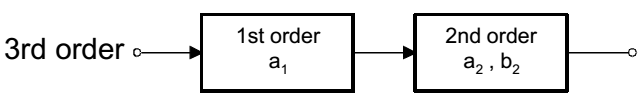
\includegraphics[scale=0.7]{figures/cProblemloesning/Filter_Orden.PNG}
	\caption{På figuren ses, hvordan et $3$. ordens lavpasfilter designes ved et $1$. og $2$. ordens lavpasfilter i forlængelse af hinanden. Værdierne $a_{1}$, $a_{2}$ og $b_{2}$ er fastsatte værdier, som kan aflæses i en tabel for Butterworth koefficienterne. \cite{Carter2013}}
	\label{fig:filter_Orden}
\end{figure}
\noindent% $3$. ordens filtret designes efter SKT-metoden bestående af tre modstande, tre kondensatorer og to operationsforstærkere. 
Et $1$. ordens lavpasfilter skal benytte en modstand, kondensator og operationsforstærker, hvoraf værdien for modstanden kan udregnes ved \eqref{eq:Lavpas1Modstande}. I \eqref{eq:LavpasModstande} udregnes modstandene for et $2$. ordens lavpasfilter, som skal benytte to modstande, to kondensatorer og en operationsforstærker. \cite{Carter2013}
\begin{eqnarray} \label{eq:Lavpas1Modstande}
R_{1} = \frac{a_1}{2 \cdot \pi \cdot f_c \cdot C_1} \\ 
\label{eq:LavpasModstande}R_{2,3} = \frac{a_2 \cdot C_3 \pm \sqrt{{a_2}^2 \cdot C_3^2 - 4 \cdot b_2 \cdot C_2 \cdot C_3}}{4 \pi \cdot f_c \cdot C_2 \cdot C_3}
\end{eqnarray}
\noindent Værdien for $C_{1}$ i \eqref{eq:Lavpas1Modstande} og \textbf{\ref{eq:LavpasModstande}} er nødvendigvis ikke den samme, da disse to ligninger er uafhængige af hinanden. Der aflæses i en tabel for Butterworth koefficienterne, at $a_{1}$, $a_{2}$ og $b_{2}$ skal være $1$. For at finde reelle værdier under kvadratroden i \eqref{eq:LavpasModstande} skal følgende være opfyldt:
\begin{equation} \label{eq:kondensator}
C_3 \geq C_2 \frac{4 \cdot b_2}{a_2^2}
\end{equation}
\noindent I \eqref{eq:LavpasModstande} er C$1$-C$3$ kondensatorer, R$1$-R$3$ er modstande og $a_1$ og $b_1$ er konstanter, mens $f_c$ er den valgte pasbåndsfrekvens i Hz, jævnfør kravspecifikationerne afsnit \ref{FilterAfs}, side \pageref{FilterAfs}. 

\noindent For at udregne modstandene fastsættes $C_1$ til $100$nF for hhv. både $1$. og $2$. ordens lavpasfiltrene. Når $C_1$ er bestemt, kan $C_2$ for $2$. ordens lavpasfilteret beregnes ved at benytte \eqref{eq:kondensator}. %Som grundregel skal $C_3$ være over dobbelt så stor som $C_2$:
\begin{equation}  
C_3 \geq 100\text{nF} \frac{4\cdot 1}{1^2} \Rightarrow C_3 \geq 400\text{nF}
\end{equation}

\noindent Ud fra ovenstående ligning vælges $C_3$ til at være $470$nF for at opfylde \eqref{eq:kondensator} og er derudover til rådighed i laboratoriet. Når værdierne for C er bestemt, kan modstandene for filteret bestemmes. For et $1$. ordens lavpasfilter benyttes \eqref{eq:Lavpas1Modstande} til at beregne $R_1$ og for et $2$. ordens lavpasfilter anvendes \eqref{eq:2ordenmodstand} for at beregne $R_2$ og $R_3$. 
\begin{equation} \label{eq:1ordenmodstand}
R_{1} = \frac{1}{2 \cdot \pi \cdot 25 \cdot 100nF} = 63661.9772 \Omega
\end{equation}
\begin{equation}
\label{eq:2ordenmodstand}R_{2,3} = \frac{1 \cdot 470\text{nF} \pm \sqrt{1^2 \cdot 470\text{nF}^2 - 4 \cdot 1 \cdot 100\text{nF} \cdot 470\text{nF}}}{4 \pi \cdot 25\text{Hz} \cdot 100\text{nF} \cdot 470\text{nF}} = \begin{cases} R_{2} = 19546.69414 \Omega \\ R_{3} =  44115.28306 \Omega \end{cases}
\end{equation}
\noindent Filterets værdier for kondensatorerne og modstandene er nu udregnet for hhv. $1$. og $2$. ordens filter. Filterkonfigurationen kan nu simuleres i LTspice, som ses på \figref{fig:lavpasfilter1_LTspice}, for at bestemme kvaliteten af det $3$. ordens filter, der er blevet designet.

\begin{figure}[H]
	\centering
	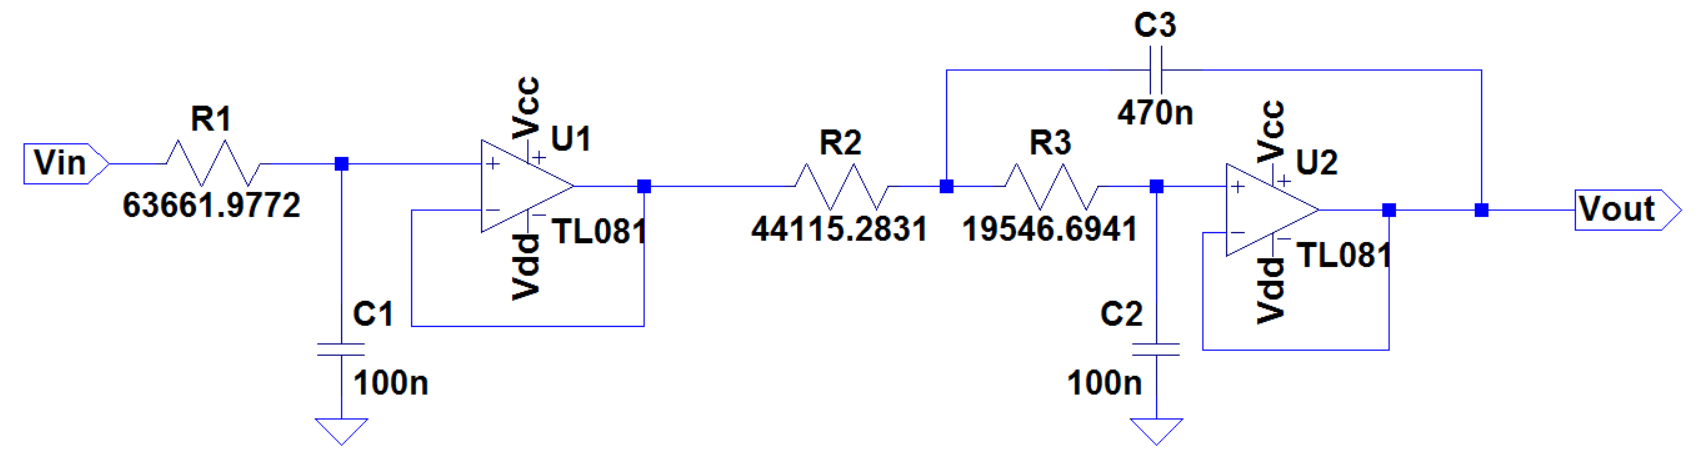
\includegraphics[scale=0.35]{figures/cProblemloesning/Lavpasfilter1_LTspice.PNG}
	\caption{På figuren ses designet af det teoretiske kredsløb for lavpasfilteret med udregnede værdier for de enkelte modstande og kondensatorer.}
	\label{fig:lavpasfilter1_LTspice}
\end{figure}

\subsubsection{Simulering}
For at udføre en simulering af $3$. ordens lavpasfilteret foretages en AC-analyse, der beskriver forholdet mellem frekvensindholdet og filterets dæmpning. Kredsløbet simuleres med et inputsignal, der har en amplitude på $1$V. I simuleringen undersøges det, hvorvidt filtret overholder kravspecifikationerne, jævnfør afsnit \ref{FilterAfs}, side \pageref{FilterAfs}, ved at betragte et bodeplot over det simulerede $3$. ordens filter.
\begin{figure}[H]
	\centering
	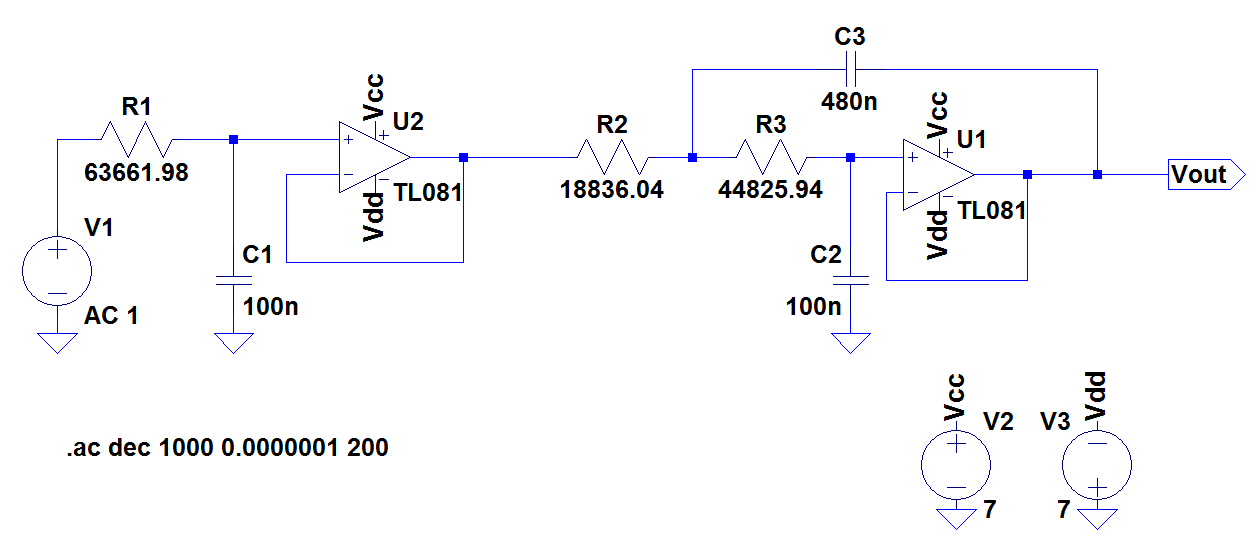
\includegraphics[scale=0.35]{figures/cProblemloesning/Lavpasfilter_LTspice.PNG}
	\caption{På figuren ses designet af $3$. ordens lavpasfilteret. Filteret simuleres vha. en AC-analyse med et inputsignal, der har en amplitude på $1$V.}
	\label{fig:lavpasfilter_LTspice}
\end{figure}
\begin{figure}[H]
	\centering
	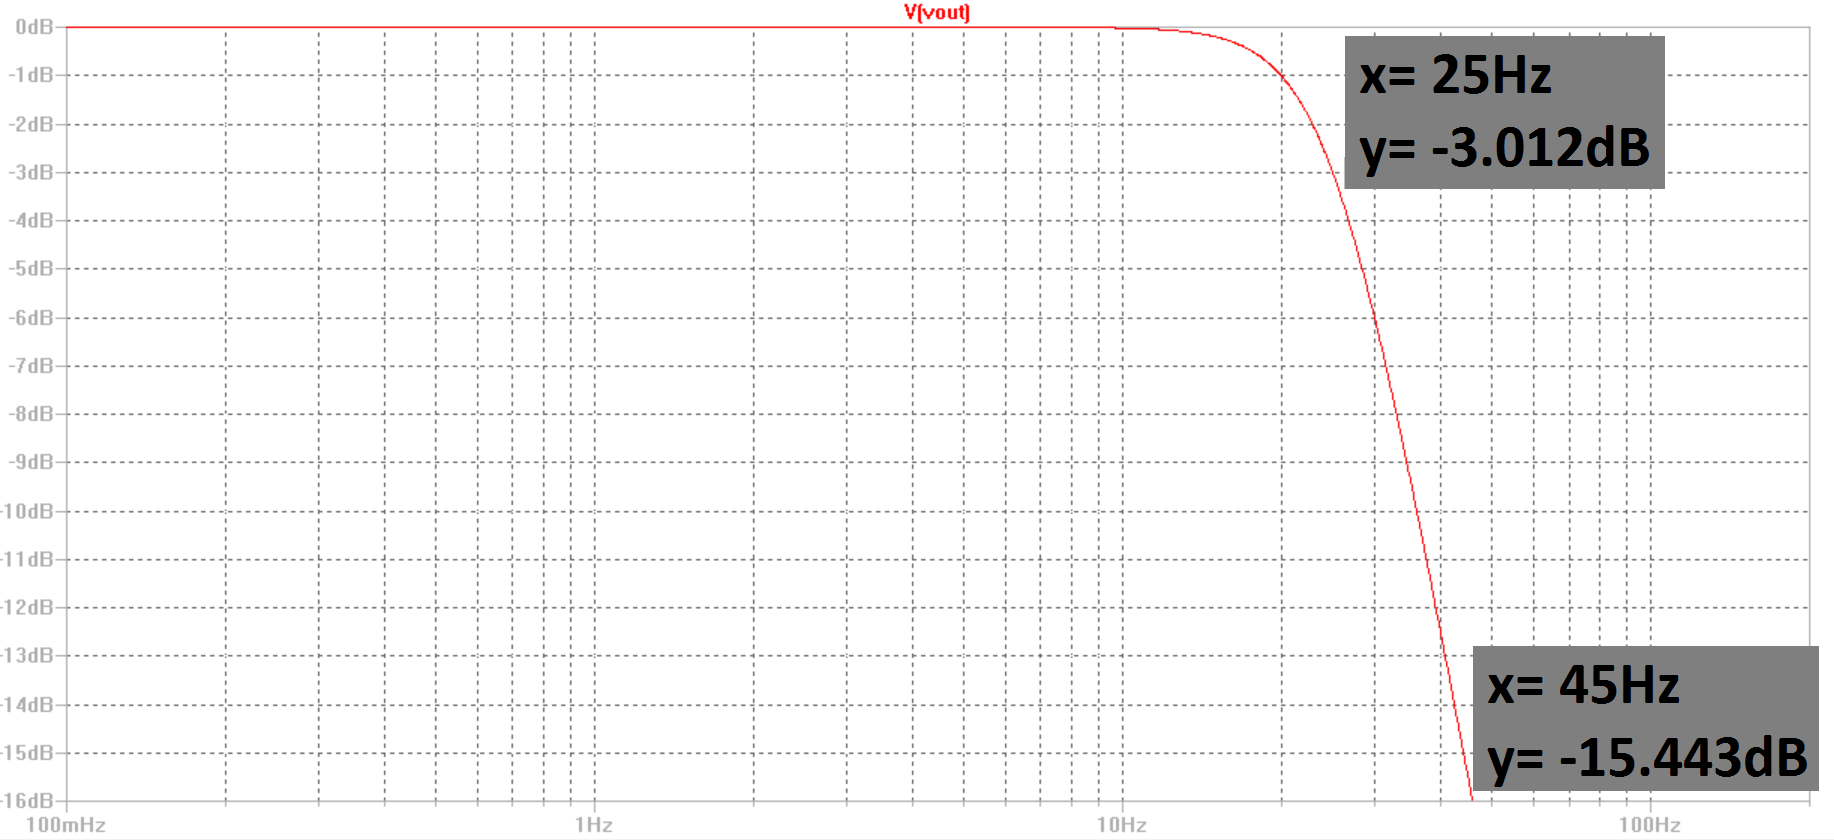
\includegraphics[scale=0.38]{figures/cProblemloesning/Lavpasfiltergraf_LTspice2.PNG}
	\caption{På figuren ses en illustration af et bodeplot, der viser $3$. ordens filterets frekvensindhold målt i Hz over dæmpningen målt i dB.}
	\label{fig:lavpasfiltergraf_LTspice1}
\end{figure}
\noindent Af \figref{fig:lavpasfiltergraf_LTspice1} fremgår det, at det simulerede filter har en maksimal dæmpning i dB på $3.012$ ved en pasbåndfrekvens på $25$Hz, hvilket ikke overholder kravspecifikationerne i afsnit \ref{FilterAfs}, side \pageref{FilterAfs}. Grundet den lave afvigelse accepteres lavpasfiltret i midlertid og der udføres derfor endnu en simulering af filteret med de reelle modstande, der benyttes under implementeringen. Der ses yderligere, at der ved en stopbåndsfrekvens på $45$Hz ses en dæmpning i dB på $15.443$. Dette overholder projektets opstillede krav for filterkonfigurationen ved en minimum dæmpning på $14$ dB i stopbåndfrekvensen.

Der ses på \figref{fig:lavpasfilter_LTspice}, at der skal benyttes tre modstande på hhv. $63661.9772\Omega$, $44115.2831\Omega$ og $19546.694\Omega$ til opbygningen af filtret. Ingen af disse modstande findes reelt, hvorfor de nærmeste alternativer er udregnet. For at få $63661.9772\Omega$ skal en $1$M$\Omega$  sættes parallelt med $68$K$\Omega$, hvilket teoretisk giver en afvigelse på $0.013\%$. For at få $44115.2831\Omega$ skal $680$K$\Omega$ sættes parallelt med $47$K$\Omega$, hvilket teoretisk giver en afvigelse på $0.349\%$. For at få en $19546.694\Omega$ sættes $39$K$\Omega$ parallelt med $39$K$\Omega$, hvilket teoretisk giver en afvigelse på $0.239\%$. Disse blev målt, hvilket ses i \tableref{Tab:Maalingafmodstande_filter}.
\begin{table}[H]
	\centering
	\begin{tabular}{|l|l|l|l|}
		\cline{2-4} \multicolumn{1}{l|}{}
		\textit{}                                     & \textit{Teoretisk} & \textit{Måling}    & \textit{Afvigelse} \\ \hline
		\multirow{2}{*}{\textit{$R_{1}$ || :}} & $1$M$\Omega$       & $1$M$\Omega$  & $0\%$           \\ \cline{2-4} 
		& $68$K$\Omega$      & $68.079$K$\Omega$ & $0.011\%$           \\ \hline
		$R1_{eq}$: & $63661.9772\Omega$ & $63633\Omega$ &  $0.046\%$ \\ \hline
		\multirow{2}{*}{\textit{$R_{2}$ || :}} & $680$K$\Omega$     & $682.840$K$\Omega$  & $0.418\%$        \\ \cline{2-4} 
		& $47$K$\Omega$      & $47.004$K$\Omega$ & $0.010\%$           \\ \hline
		$R2_{eq}$: & $44115.2831\Omega$ & $43976\Omega$ & $0.316\%$ \\ \hline
		\multirow{2}{*}{\textit{$R_{3}$ || :}} & $39$K$\Omega$      & $38.888$K$\Omega$    & $0.287\%$           \\ \cline{2-4} 
		& $39$K$\Omega$     & $39.043$K$\Omega$        & $0.108\%$           \\ \hline
		$R3_{eq}$: & $19546.694\Omega$ & $19482\Omega$  & $0.3310\%$ \\ \hline
	\end{tabular}
	\caption{I tabellen ses at de anvendte modstande afviger fra den teoretiske værdi, hvilket er forventet af reelle komponenter. Disse afvigelser kommer derved også til at have en effekt på $R_{eq}$. Det er de teoretiske værdier, som bliver benyttet i en ny simulering.}
	\label{Tab:Maalingafmodstande_filter}
\end{table}
\noindent Filterkonfigurationen med reelle modstande fremgår af \figref{fig:Sim_reel_modstande}.
\begin{figure}[H]
	\centering
	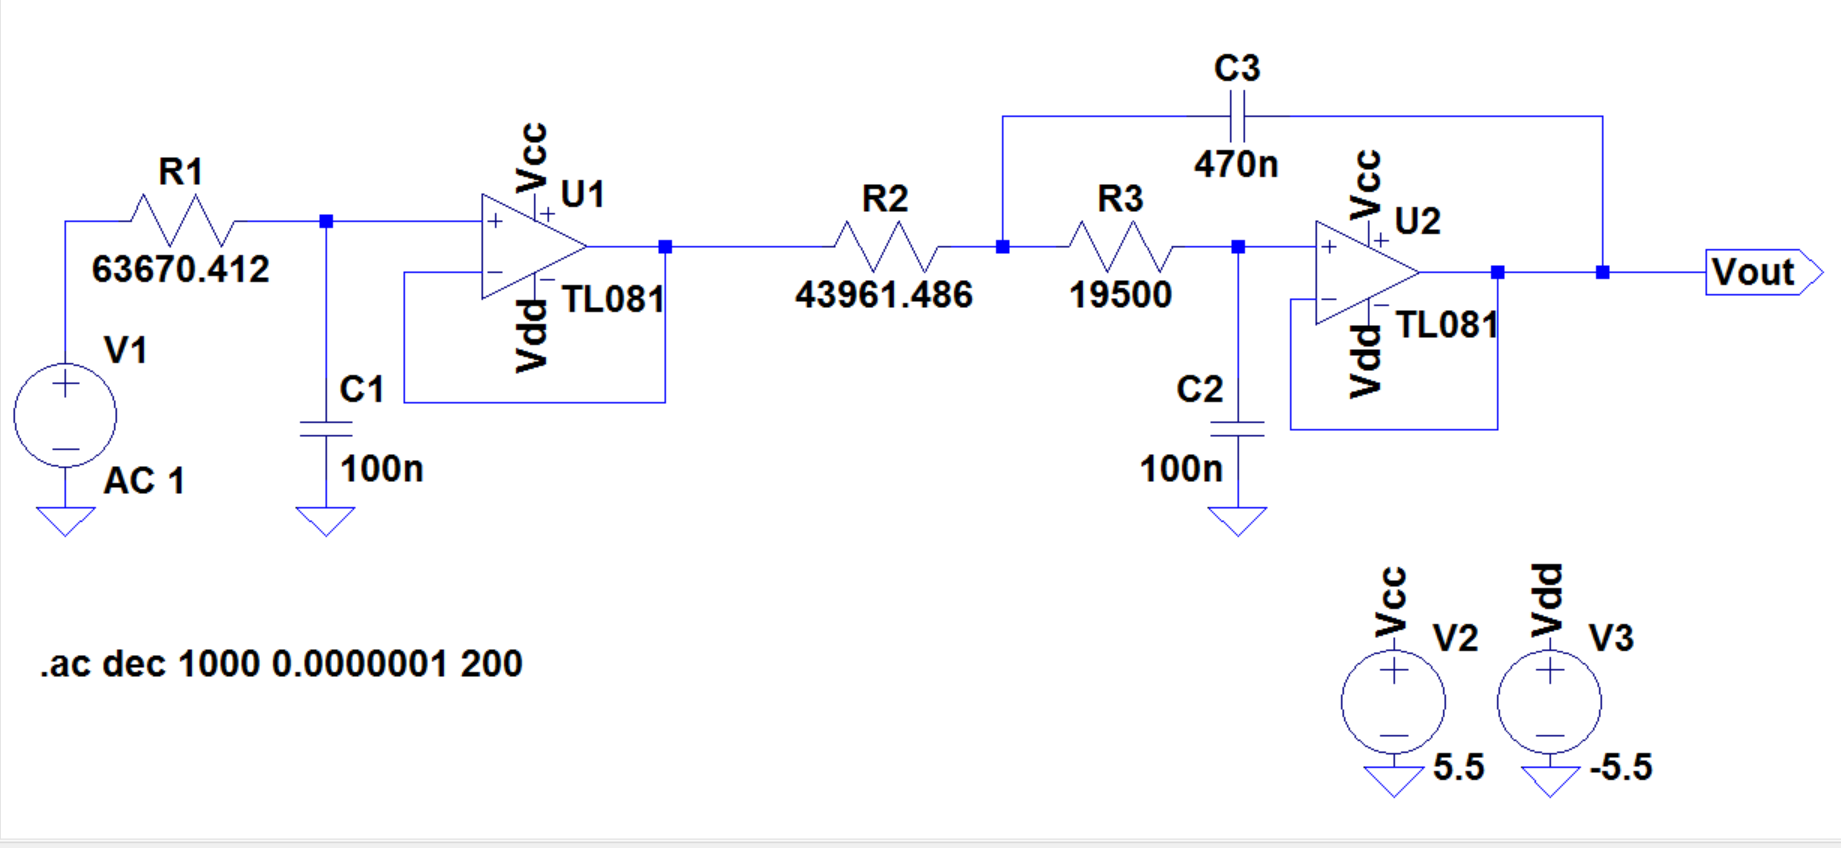
\includegraphics[scale=0.4]{figures/cProblemloesning/Sim_reel_modstande.PNG}
	\caption{På figuren ses et 3. ordens filter med modstande, som har de teoretiske $R_{eq}$ værdier - dvs. R$1$ består af en parallelforbindelse mellem $68$K $\Omega$ og $1$M $\Omega$, R$2$ består af en parallelforbindelse mellem $47$K $\Omega$ og $680$K $\Omega$ og R$3$ består af en parallelforbindelse mellem to modstande på $32$K $\Omega$.}
	\label{fig:Sim_reel_modstande}
\end{figure}

\begin{figure}[H]
	\centering
	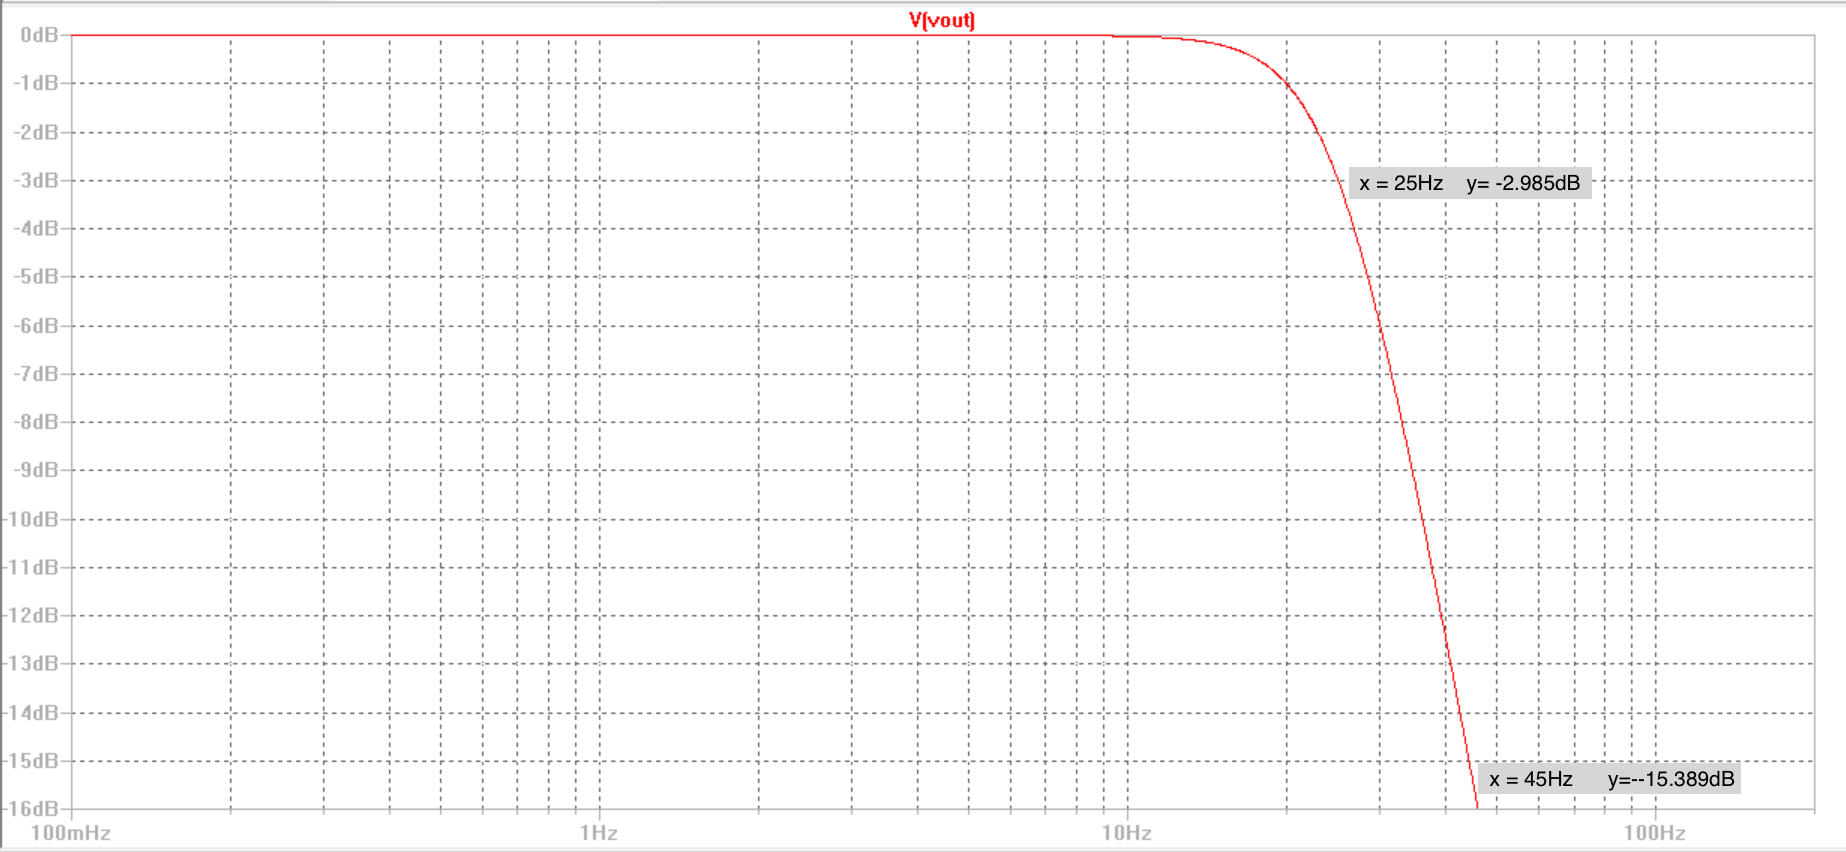
\includegraphics[scale=0.35]{figures/cProblemloesning/Sim_reel_graf.PNG}
	\caption{På figuren ses en illustration af et bodeplot, der viser 3. orden lavpasfilterets frekvensindhold målt i Hz over dæmpningen målt i dB med den teoretiske værdi for de reelle modstande.}
	\label{fig:Sim_reel_graf}
\end{figure}

\noindent Ud fra bodeplottet ses det, at det simulerede filter med reelle værdier har en maksimal amplitude på $-2.985$dB ved en pasbåndsfrekvens på $25$Hz, hvilket overholder kravspecifikationerne i afsnit \ref{FilterAfs}, side \pageref{FilterAfs}. Der aflæses, at ved stopbåndsfrekvensen på $45$Hz er amplituden $-15.389$dB, hvilket fortsat er acceptabelt ift. kravspecifikationerne for filterkonfigurationen. 

\subsubsection{Implementering og test} 
Der ses på \figref{fig:Sim_reel_modstande} at der benyttes 3 kondensatorer til at designe kredsløbet. I \tableref{Tab:Maalingafmodstande_filter} ses målingerne af de benyttede modstande. I \tableref{Tab:Maalingfilter} ses de reelle værdier for de benyttede kondensatorer.
\begin{table}[H]
	\centering
	\begin{tabular}{|l|l|l|l|}
		\hline
		\textit{$C_{1}$ :}                            & $100$n             & $98$n              & $2.00\%$           \\ \hline
		\textit{$C_{2}$ :}                            & $470$n             & $464$n             & $1.29\%$           \\ \hline 
		\textit{$C_{3}$ :}                            & $100$n             & $98$n              & $2.00\%$           \\ \hline
	\end{tabular}
	\caption{I tabellen ses, at de anvendte kondensatorer afviger fra den teoretiske værdi, hvilket er forventet af reelle komponenter. Det er en acceptabel afvigelse, hvorfor disse kan anvendes til implementering}
	\label{Tab:Maalingfilter}
\end{table}
\noindent Herefter implementeres kredsløbet. I testen anvendes en funktionsgenerator som inputsignal, og et multimeter til aflæsning af dæmpningen. Funktionsgeneratoren sættes til de ønskede frekvenser i intervaller af $1$Hz fra $10$Hz til $50$Hz. Multimeteret måler dæmpningen af signalet ved at indstille et referencepunkt ved inputspændingen. Referencepunktet sættes det sted på signalet, hvor spændingen ændrer sig mindst, hvilket sker ved $10$Hz. Referencen opfattes som signalets input. Herefter beregner multimeteret forskellen mellem input- og outputspændingen og beregner dæmpningen i dB ved samme princip som i \eqref{eq:daempningsfaktoridB}, side \pageref{eq:daempningsfaktoridB}. Outputtet fra multimetret måles for hver frekvens og noteres. Ud fra disse målinger plottes en graf af dæmpningen i MATLAB, hvilket er illustreret på \figref{fig:Lavpas_Matlab}.  

\begin{figure}[H]
	\centering
	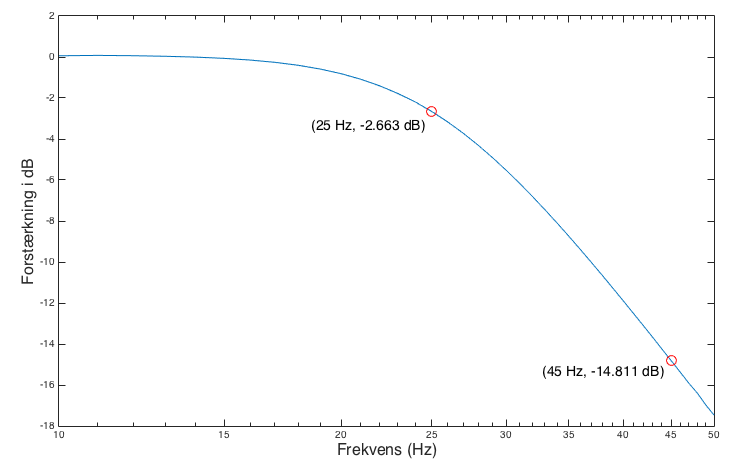
\includegraphics[scale=0.5]{figures/cProblemloesning/Lavpas_Matlab.PNG}
	\caption{På figuren ses dæmpningen som en graf over de målte frekvenser i Hz som funktion af outputtet i dB. På grafen er der angivet pasbåndfrekvens og stopbåndfrekvens.}
	\label{fig:Lavpas_Matlab}
\end{figure}

\begin{table}[H]
	\centering
	\begin{tabular}{|l|l|l|l|}
		\cline{2-4} \multicolumn{1}{l|}{}
		& \textit{Krav for dæmpning i dB} 	& \textit{Test af dæmpning i dB}  &\textit{Afvigelse} \\ \hline
		\textit{Pasbåndsfrekvens} & $3$	& $2.7360$	    & $8.8\%$ \\ \hline
		\textit{Stopbåndsfrekvens} & $14$    & $14.8480$    & $6.1\%$  \\ \hline
	\end{tabular}
	\caption{I tabellen ses afvigelserne for dæmpningen i pasbånds- og stopbåndsfrekvensen ift. kravspecifikationerne og den fortagede test.}
	\label{Tab:Tolerance}
\end{table}
\noindent Ud fra de testede værdier i \tableref{Tab:Tolerance} ses en afvigelse på pasbånds- og stopbåndsfrekvensen ift. kravet for dæmpning kravspecifikationer i afsnit \ref{FilterAfs}, side \pageref{FilterAfs}. Dæmpningen i pasbåndsfrekvensen skal maksimalt være $3$dB, hvilket betyder, at testen ligger indenfor tolerancekravet med en dæmpning i pasbåndet på $2.7$dB. Derudover skal lavpasfilteret dæmpe med minimum $14$dB i stopbåndsfrekvensen. Denne tolerance overholdes i testen med en dæmpning på $14.8480$dB, hvorfor filterblokken accepteres.\\

\noindent\textbf{Sammenligning mellem det simulerede og implementerede lavpasfilter} \\
\noindent På \figref{fig:sammenligning_sim_imp} er afvigelsen for det simulerede lavpasfilter ift. det implementerede lavpasfilter visualiseret vha. et bodeplot. 
\begin{figure}[H]
	\centering
	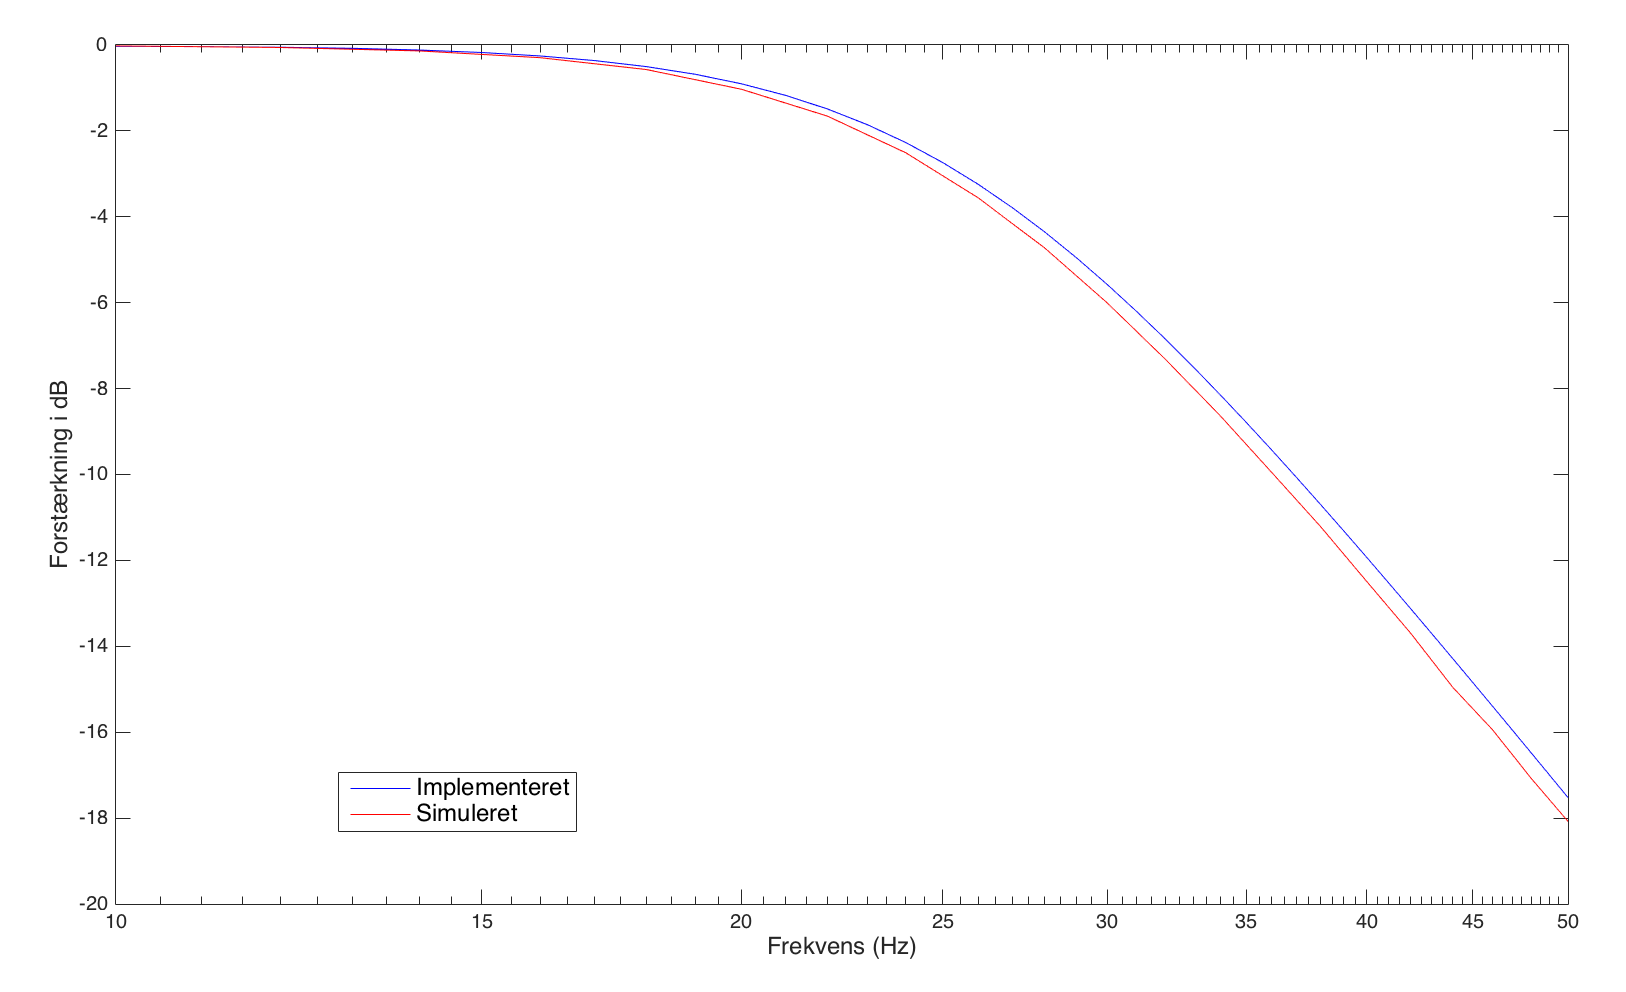
\includegraphics[scale=0.4]{figures/cProblemloesning/sammenligning_sim_imp.PNG}
	\caption{På figuren ses et bodeplots for det simulerede lavpasfilter, markeret med rød, og et bodeplot for det implementerede lavpasfilter, markeret med blå.}
	\label{fig:sammenligning_sim_imp}
\end{figure}
\noindent Bodeplottet for det simulerede lavpasfilter er udarbejdet ud fra $20$ målepunkter og det implementerede er udarbejdet ud fra $40$ målepunkter i intervallet $10$ til $50$Hz. Det fremgår af \figref{fig:sammenligning_sim_imp}, at der er forskel mellem at konstruere et teoretisk lavpasfilter og implementere et. Det er ikke muligt at implementere et lavpasfilter, der er ens med det simulerede grundet reelle komponenters afvigelse. Det fremgår, at det simulerede lavpasfilter ligger under det implementerede lavpasfilter, hvilket stemmer overens med at dæmpningsværdien er højere i det simulerede ift. det implementerede. \\
Der ses ud fra testen og sammenligningen, at lavpasfilteret overholder kravspecifikationerne i afsnit \ref{FilterAfs}, side \pageref{FilterAfs}. Derudover ligger afvigelserne indenfor tolerancekravene og derfor accepteres lavpasfilteret. 